\newpage
\changeindent{0cm}
\section{提案手法}
\changeindent{2cm}

本章では,本研究の提案手法について説明する.

\changeindent{0cm}
\subsection{漫画のセリフのマルチモーダルな感情推定手法}
\changeindent{2cm}

本研究では, 4 コマ漫画ストーリーデータセットを用いて,
各セリフにアノテートされた感情ラベルを推定するタスクを解き, その精度を確認する.

図 \ref{fig:teian} にマルチモーダルな推定手法として, 提案手法の概要を示す.
Text Embedding 層への入力として, あるセリフを選んだ時に, Image Embedding 層への入力をこのセリフが含まれているコマの画像全体とする. そして, それぞれの層から得たものをセリフベクトルとコマベクトルとし, これらを結合したものを識別器への入力とすることでセリフの感情ラベルを推定する.

\begin{figure}[h]
  \centering
  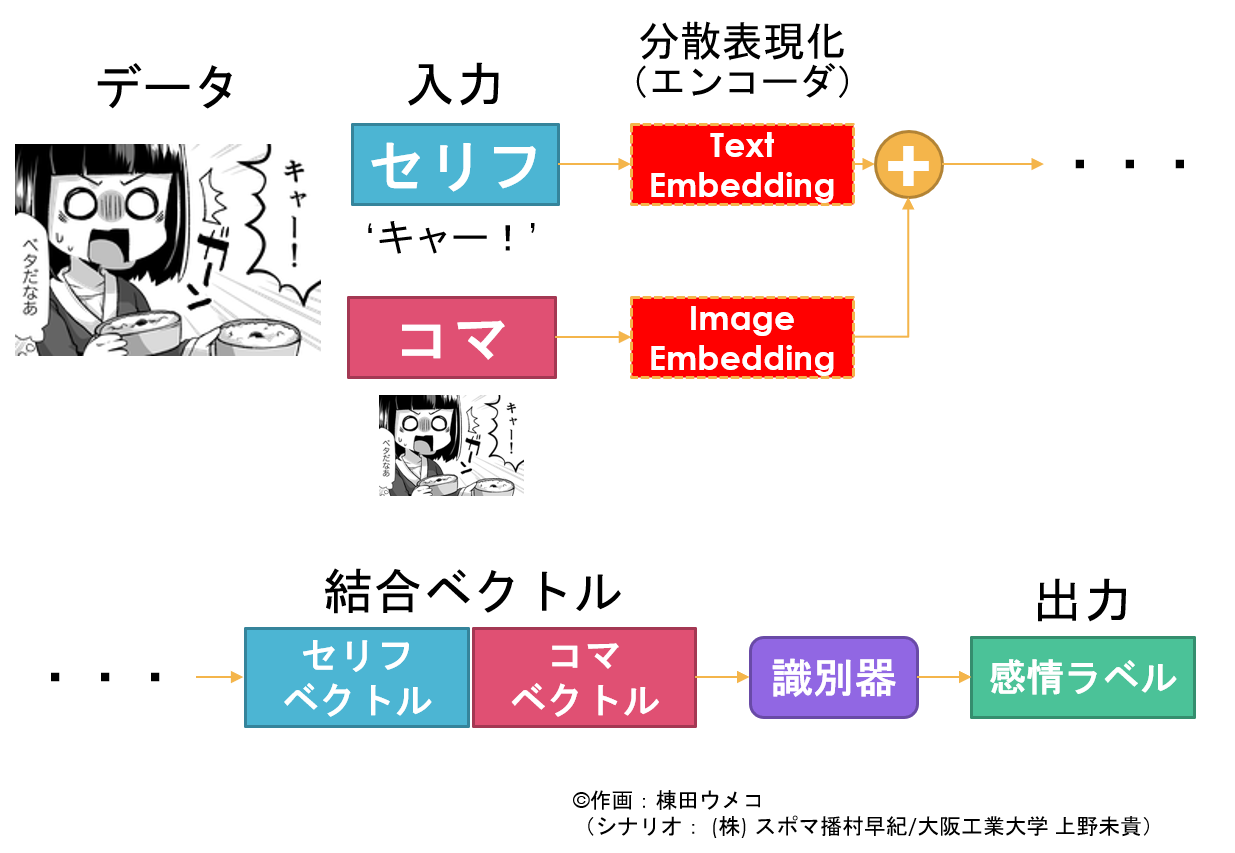
\includegraphics[width=0.8\hsize]{doc/figures/teian_2.png}
  \caption{提案手法の概要}
  \label{fig:teian}
\end{figure}

\newpage
\changeindent{0cm}
\subsection{Data Augmentation}
\changeindent{2cm}

4 コマ漫画ストーリーデータセットの欠点として, データ数が少ないことがあげられる.
そこで, 本研究では日本語 WordNet \cite{word_net_jp} のシソーラスを用いてテキストデータを拡張する.

図 \ref{fig:data_aug} に Data Augmentation の概要を示す.
分かち書きされたオリジナルのセリフに対して, 日本語 WordNet で類似語を持つ単語について類似語に置き換え, 文を生成することでテキストデータを拡張した. ただし, 文の中に類義語を持つ単語が
複数あった場合, 類似語に置き換える単語は同時に 1 つまでとし, 英数字・記号のみで表されている類似語は除外した. 例えば, 5 つの単語からなる文章があり,
各単語が 5 つの類似語を持っている場合, その文からは新しく 25 文が生成されることとなる.

\begin{figure}[h]
  \centering
  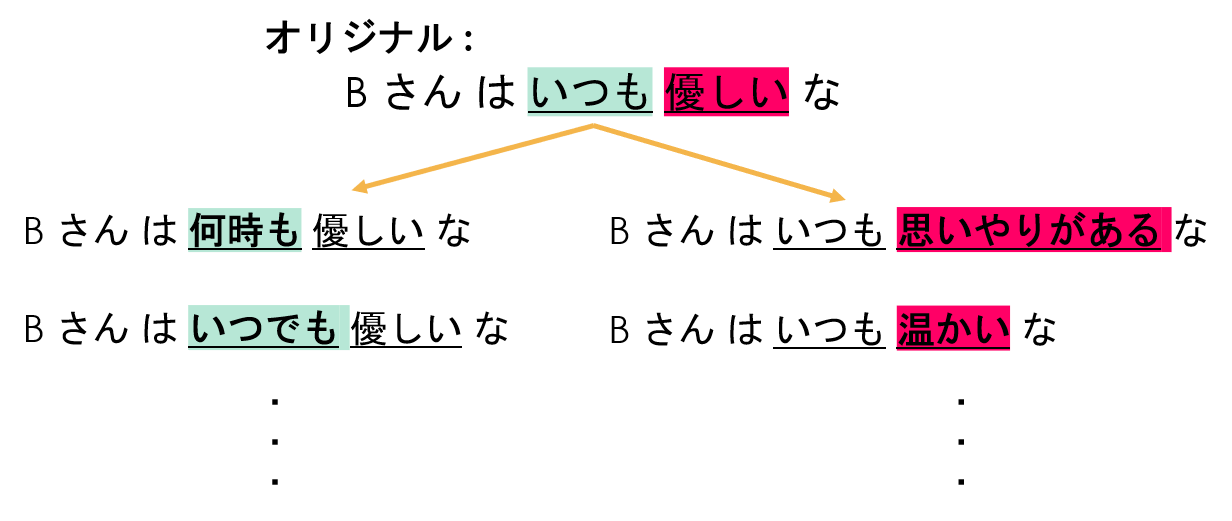
\includegraphics[width=0.8\hsize]{doc/figures/data_aug.png}
  \caption{Data Augmentation の概要}
  \label{fig:data_aug}
\end{figure}
